%-------------------------------------------------------------------------------------------------------------------------------%
%*******************************************************************************************************************************%
%************************************************** Dissertation-Schultze.tex **************************************************%
%*******************************************************************************************************************************%
%-------------------------------------------------------------------------------------------------------------------------------%
\documentclass{thesis}
%-------------------------------------------------------------------------------------------------------------------------------%
\usepackage{epsfig}                 %% Permit the use of postscript figures within the document.
%\patchcmd{\Ginclude@eps}{"#1"}{#1}{}{}
%_______________________________________________________________________________________________________________________________%
%*******************************************************************************************************************************%
%===============================================================================================================================%
%-------------------------------------------------- Dissertation-Prologue.tex --------------------------------------------------%
%===============================================================================================================================%
%*******************************************************************************************************************************%
% File: Dissertation-Prologue.tex
% Description: this file is where the abstract, acknowledgements, dedication, and attributions should be defined AND/OR excluded.
% Usage: + Fill in the \X{...} macros that you want to be INCLUDED in your document; this automatically sets the corresponding
%        \if@makeXPage conditional to TRUE and inserts the associated \thesisXPage into the document in the proper order.     
%        + To EXCLUDE any of these frontmatter pages from the document, uncomment the corresponding \excludeX macros. Commenting
%        out the \X{...} macro will also prevent the corresponding Page from being included in the document.
%
%
%_______________________________________________________________________________________________________________________________%
% Last Updated in December, 2023
%_______________________________________________________________________________________________________________________________%
%===============================================================================================================================%
%------------------------------------------------------ Prologue Controls ------------------------------------------------------%
%===============================================================================================================================%
%\makeCopyrightPage
%\makeListOfFigures
%\makeListOfTables
%-------------------------------------------------------------------------------------------------------------------------------%
%\excludeAbstractPage
%\excludeAcknowlegmentsPage
%\excludeDedicationPage
%\excludeAttributionsPage
%\emptyLoT                                                              % Tell latex that there is no list of tables
%-------------------------------------------------------------------------------------------------------------------------------%
%\setUppercaseHeadings
%\setCapitalizedHeadings
%-------------------------------------------------------------------------------------------------------------------------------%
%\setUppercaseToCtitles
%\setCapitalizedToCtitles
%-------------------------------------------------------------------------------------------------------------------------------%
%\setLoZtitlesAligned
%\setLoZtitlesConstsep
%-------------------------------------------------------------------------------------------------------------------------------%
%\cftsetindents{figure}{0in}{\len@p@figure}                                      % Increase the width of the figure number line box to contain "Figure X.XX", but reduce the gap before subsequent title by 1em to ~1 space DEFAULT:{1.5em}{2.3em}
%\cftsetindents{table}{0in}{\len@p@table}                                        % Increase the width of the table number line box to contain "Table X.XX", but reduce the gap before subsequent title by 1em to ~1 space DEFAULT:{1.5em}{2.3em}
%\cftsetindents{chapter}{0in}{0in}
%\cftsetindents{section}{\cftindent@between@chap@sec}{0in}
%\cftsetindents{subsection}{\cftindent@between@chaplines+\cftindent@between@any@sec*2}{0in}
%\cftsetindents{subsubsection}{\cftindent@between@chaplines+\cftindent@between@any@sec*3}{0in}
%\cftsetindents{paragraph}{\cftindent@between@chaplines+\cftindent@between@any@sec*4}{0in}
%_______________________________________________________________________________________________________________________________%
%*******************************************************************************************************************************%
%===============================================================================================================================%
%--------------------------------------------------------- FRONTMATTER ---------------------------------------------------------%
%-------------------------------------------------------------------------------------------------------------------------------%
%----------------------------------------- Frontmatter (Prologue) page(s) text content -----------------------------------------%
%===============================================================================================================================%
%*******************************************************************************************************************************%
%_______________________________________________________________________________________________________________________________%
%===============================================================================================================================%
%---------------------------------------------------------- Abstract -----------------------------------------------------------%
%===============================================================================================================================%
\abstract{The work presented in this dissertation...
}
%===============================================================================================================================%
%------------------------------------------------------ Acknowledgements -------------------------------------------------------%
%===============================================================================================================================%
\acknowledgements{Special thanks go to...
}
%===============================================================================================================================%
%--------------------------------------------------------- Dedication ----------------------------------------------------------%
%===============================================================================================================================%
%-------------------------------------------------------------------------------------------------------------------------------%
%\setDedicationFontstyle{it}
%\setPageFontstyle{Dedication}{bf}
%-------------------------------------------------------------------------------------------------------------------------------%
\dedication{This is dedicated to...
}
%===============================================================================================================================%
%-------------------------------------------------------- Attributions ---------------------------------------------------------%
%===============================================================================================================================%
%-------------------------------------------------------------------------------------------------------------------------------%
% Example usage of the \attributions macro and the associated 'attributionList', 'attribution', and 'authorList' environments
% designed to generate an appropriately formatted attributions list.
%-------------------------------------------------------------------------------------------------------------------------------%
\attributions{%
\begin{attributionList}
%-------------------------------------------------------------------------------------------------------------------------------%
    \item\begin{attribution}
        %Schultze, B. E., M. Witt, Y. Censor, K. E. Schubert, and R. W. Schulte (2015). Performance of hull-detection algorithms for proton computed tomography reconstruction. In S. Reich and A. Zaslavski (Eds.), \textit{Infinite Products of Operators and Their Applications}, Volume 636 of \textit{Contemporary Mathematics}, pp. 211–224. American Mathematical Society.
         B. E. Schultze, M. Witt, Y. Censor, K. E. Schubert, and R. W. Schulte, “Performance of hull-detection algorithms for proton computed tomography reconstruction,” in \textit{Infinite Products of Operators and Their Applications}, ser. Contemporary Mathematics, S. Reich and A. Zaslavski, Eds., vol. 636. American Mathematical Society, 2015, pp. 211–224.
    \end{attribution}\label{attribution:hull-detection}%
    \begin{authorList}
        \item I (B. E. Schultze) was the sole investigator and primary author of the publication.
        \item M. Witt provided the simulated data sets used for the initial hull-detection investigations.
        \item Y. Censor, K. E. Schubert, and R. W. Schulte acted in a supervisory role on editing, content accuracy, and approval of the final form submitted for publication.
    \end{authorList}
%-------------------------------------------------------------------------------------------------------------------------------%
    \item\begin{attribution}%
        %Schultze, B. E., Y. Censor, P. Karbasi, K. E. Schubert, and R. W. Schulte (2020). An Improved Method of Total Variation Superiorization Applied to Reconstruction in Proton Computed Tomography. \textit{IEEE Transactions on Medical Imaging 39}(2), 294–307.
        B. E. Schultze, Y. Censor, P. Karbasi, K. E. Schubert, and R. W. Schulte, “An Improved Method of Total Variation Superiorization Applied to Reconstruction in Proton Computed Tomography,” \textit{IEEE Transactions on Medical Imaging}, vol. 39, no. 2, pp. 294–307, 2020
    \end{attribution}\label{attribution:ntvs}
    \begin{authorList}
        \item I (B. E. Schultze) was the sole investigator and primary author of the publication.
        \item Y. Censor is among the original developers of the superiorization methodology, which serves as the theoretical framework of total variation superiorization, and requested the investigations be performed for pCT. He also provided approval of the investigation results and final form submitted for publication.
        \item P. Karbasi was a colleague working independently on a related topic who participated in discussions to ensure our investigations did not overlap. She also assisted in the editing of the final form submitted for publication.
        \item K. E. Schubert and R. W. Schulte acted in a supervisory role on editing, content accuracy, and approval of the final form submitted for publication.%
    \end{authorList}%
\end{attributionList}
}
%_______________________________________________________________________________________________________________________________%
%*******************************************************************************************************************************%
%===============================================================================================================================%
%----------------------------------------------- END: Dissertation-Prologue.tex ------------------------------------------------%
%===============================================================================================================================%
%*******************************************************************************************************************************%
\endinput

\graphicspath{{./images/}}
%-------------------------------------------------------------------------------------------------------------------------------%
\title{Title of Your Dissertation}                                      %\thesisTitle

\author{John G. Student}                                                %\thesisAuthor
\holding{B.S., M.S.}                                                    %\thesisHolding
\seeking{Ph.D.}                                                         %\thesisSeeking
\degree{Doctor of Philosophy}                                           %\thesisDegree

\department{Department of Electrical and Computer Engineering}          %\thesisDepartment
\departmentChair{Your D. Chair, Ph.D.}                                   %\thesisDepartmentChair
%\schoolChair{Kwang Y. Lee, Ph.D.}
\graduateDean{Your D. Dean, Ph.D.}                                     %\thesisDean
\supervisor{Chairperson Name, Ph.D.}                                    %\thesisMentor
\supervisorTitle{Mentor}                                                %\thesisMentorTitle
\readerOne{Reader One, Ph.D.}                                           %\thesisReaderOne
\readerTwo{Reader Two,  Ph.D.}                                          %\thesisReaderTwo
\readerThree{Reader Three, Ph.D.}                                       %\thesisReaderThree
\date{Grad-Month Grad-Year}                                             %\thesisConfDate

% If you acquired signatures on a separate PDF, uncomment this line and change the PDF title as needed
%\insertSignaturePage{./SignaturesPage.pdf}

\makeListOfFigures                                                      % sets \@makeLoFtrue-> adds \thesisLoFpage to \thesisPrologue
\makeListOfTables                                                       % sets \@makeLoTtrue-> adds \thesisLoTpage to \thesisPrologue


%\emptyLoT                                                              % Tell latex that there is no list of tables
%\excludeAbstractPage
%\excludeAcknowlegmentsPage
%\excludeDedicationPage
%\excludeAttributionsPage
%-------------------------------------------------------------------------------------------------------------------------------%
%*******************************************************************************************************************************%
%****************************************************** MAIN DOCUMENT BODY *****************************************************%
%*******************************************************************************************************************************%
%-------------------------------------------------------------------------------------------------------------------------------%
\begin{document}
	
%-------------------------------------------------------------------------------------------------------------------------------%
%*******************************************************************************************************************************%
%******************************************************** C1-Intro.tex *********************************************************%
%*******************************************************************************************************************************%
%-------------------------------------------------------------------------------------------------------------------------------%
\chapter[Intro]{Introduction (Level 2)}\label{chap:intro}

Overview of dissertation: motivation, the reason more work is needed, the importance of your work and how it addresses this need, and a topical overview of what will be presented in the following chapters.

\section{First section (Level 3)}

Some first section text
\subsection{First subsection (Level 4) of First Section (Level 3)}

Some first subsection text
\subsubsection{First subsubsection (Level 5) of First Subsection (Level 4)}

Some first subsubsection text
\section{Second Section (Level 3)}
\subsection{First subsection (Level 4) of Second Section (Level 3)}
\subsubsection{First subsubsection (Level 5) of Second Subsection (Level 4)}
\section*{Third section (Level 3): unnumbered \textbackslash section* variant}
%
This section appears in the main document body here but \textbackslash section* (1) generates an UNNUMBERED section heading
and (2) DOES NOT create a corresponding ToC list item.

The same behavior is true for \textbackslash subsection* and \textbackslash subsubsection*.
%-------------------------------------------------------------------------------------------------------------------------------%
%*******************************************************************************************************************************%
%******************************************************** C1-Intro.tex *********************************************************%
%*******************************************************************************************************************************%
%-------------------------------------------------------------------------------------------------------------------------------%
\endinput 
	\begin{figure}
	  \centering
	  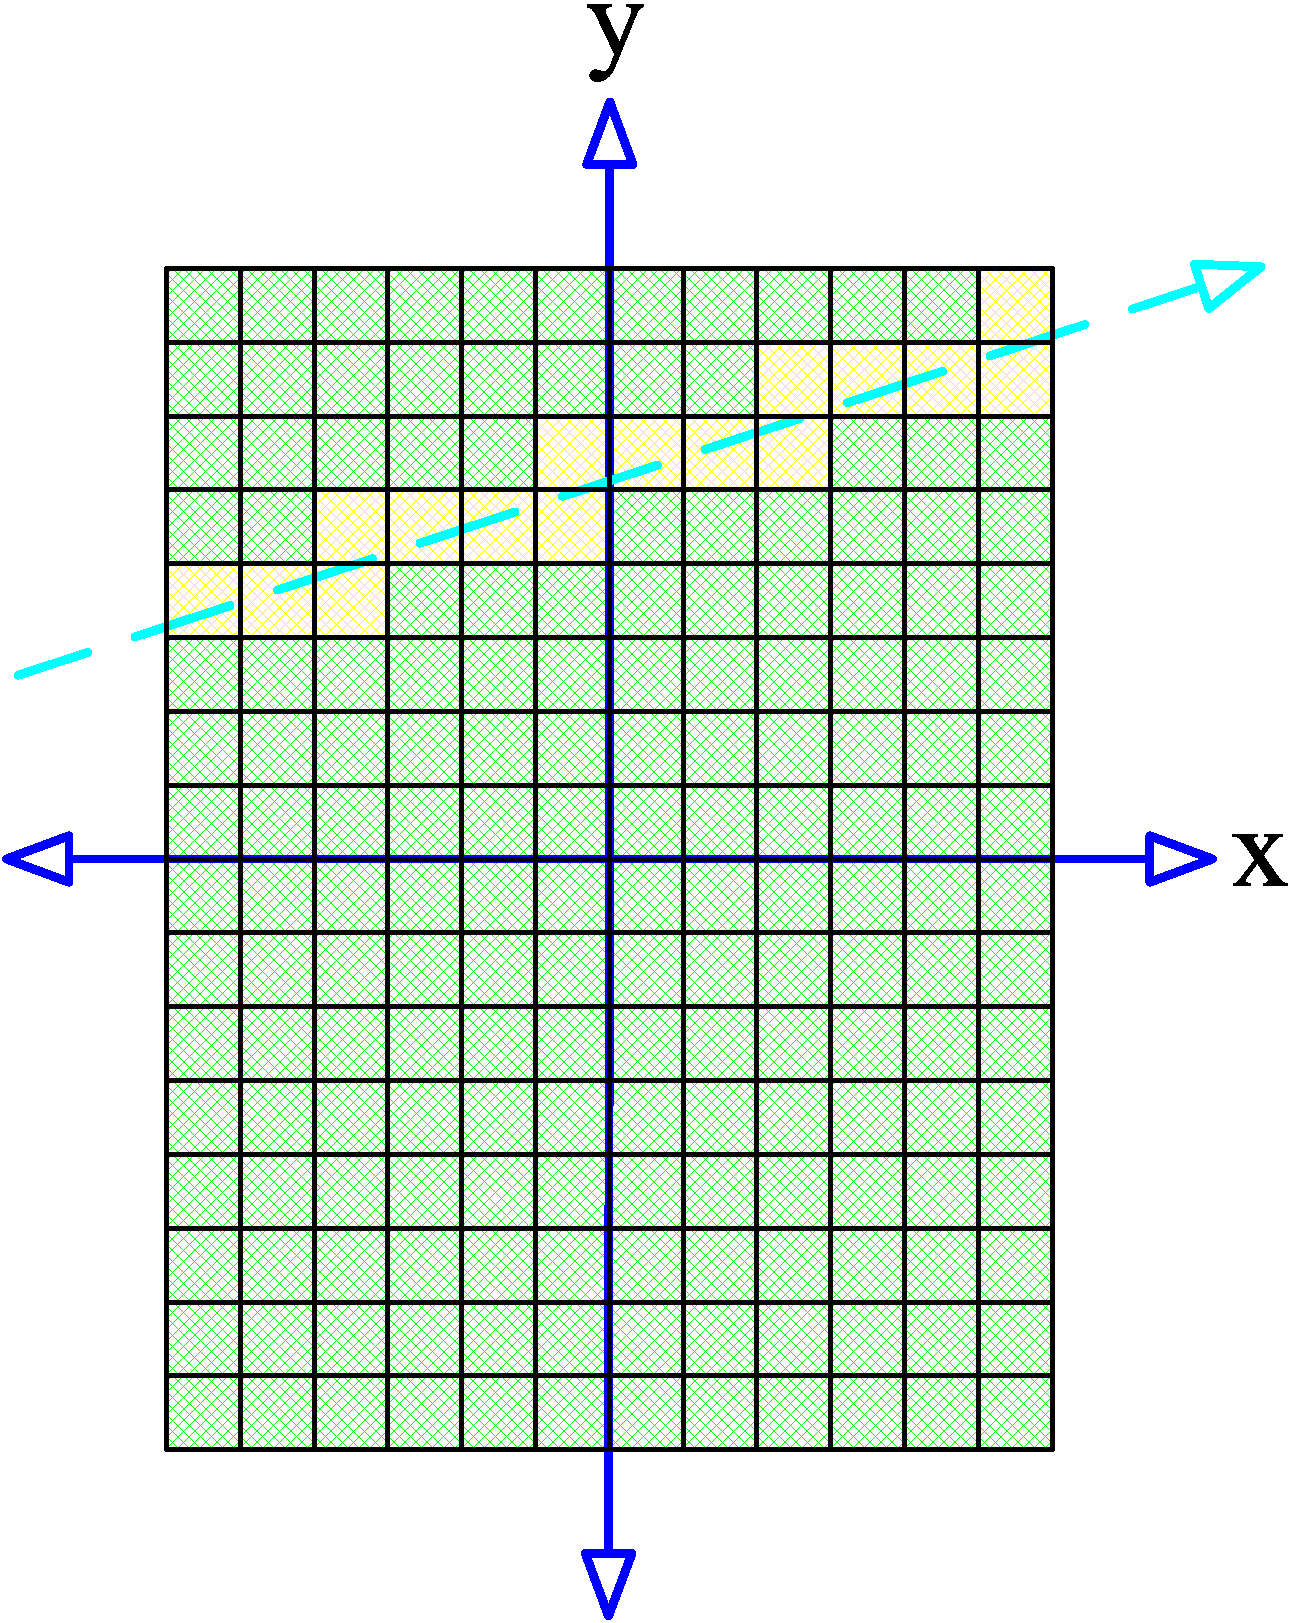
\includegraphics[width=4cm]{Space_Carving_1.png}
	  \caption{Hello DDA figure caption }\label{fig:DDA}
	\end{figure}
	\begin{figure}
	  \centering
	  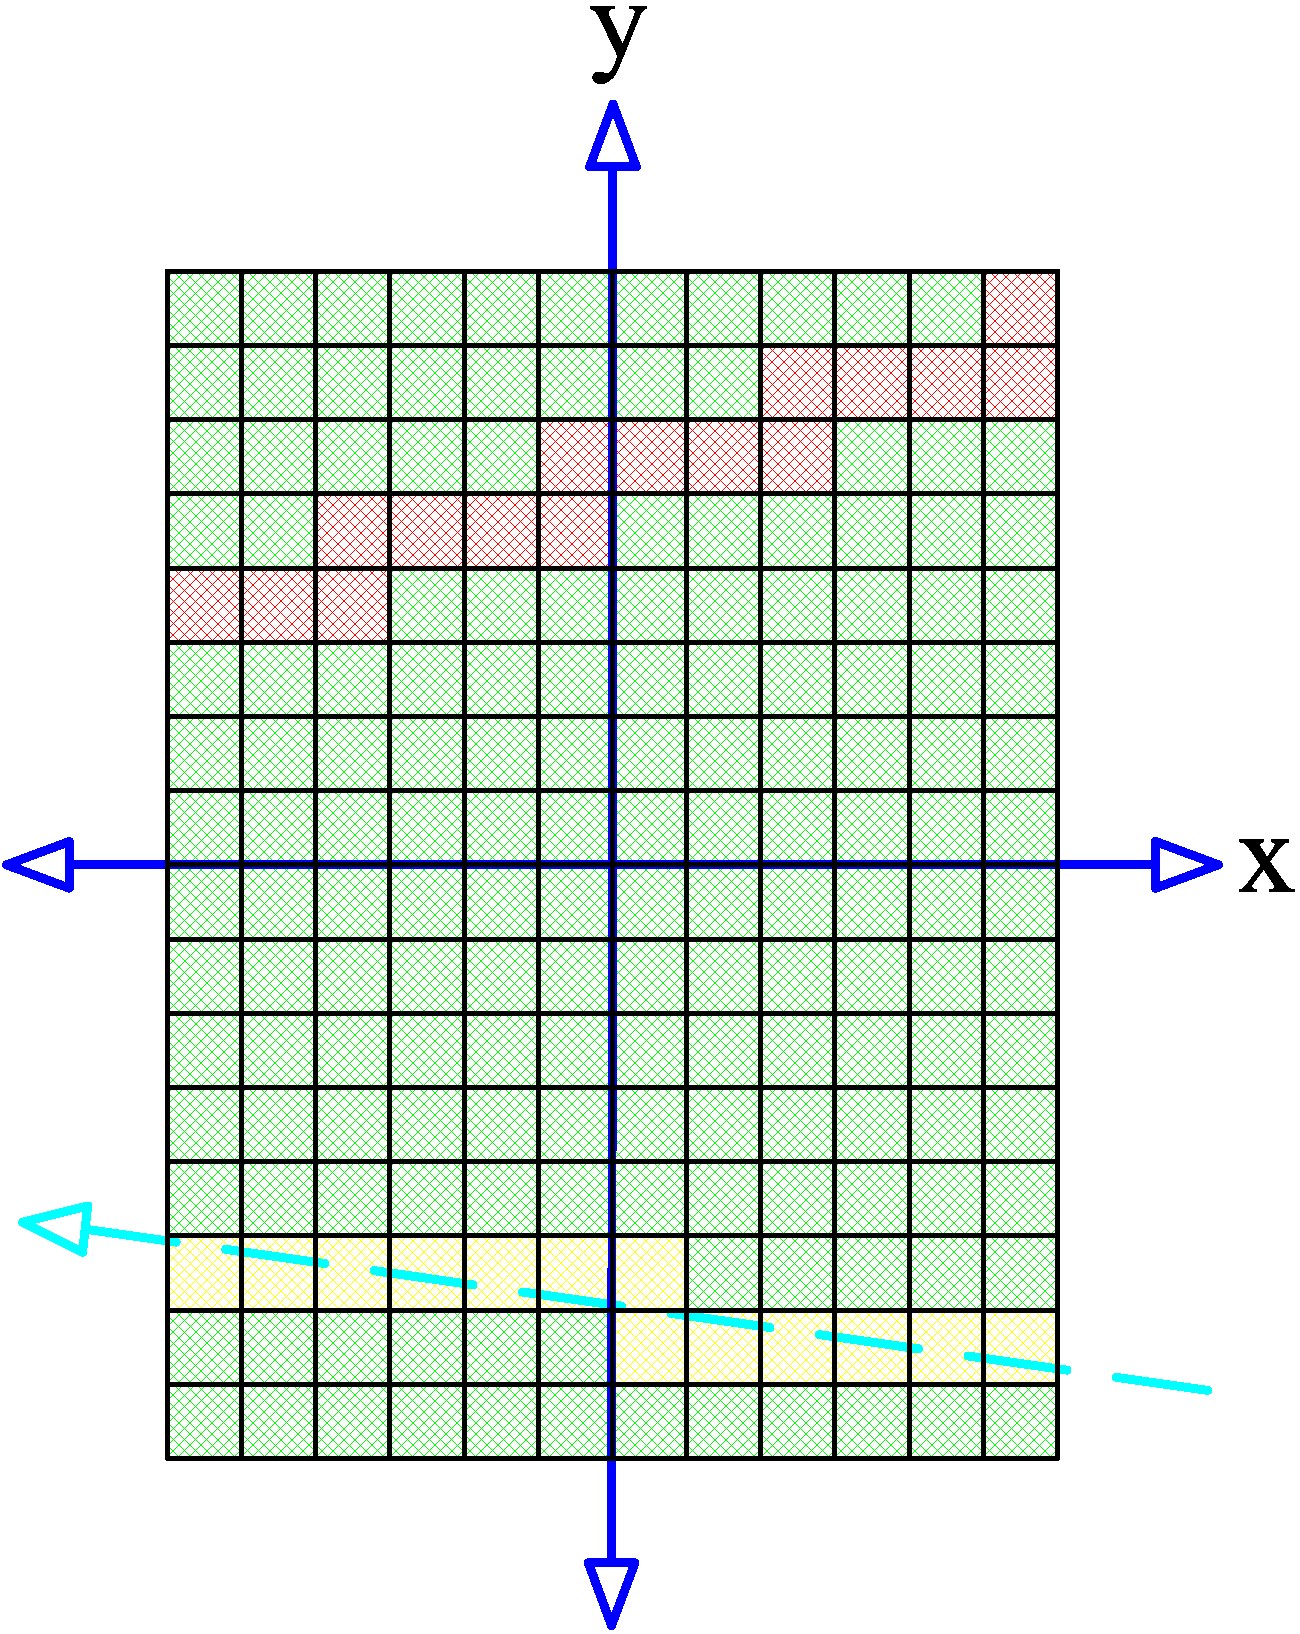
\includegraphics[width=4cm]{Space_Carving_2.png}
	  \caption{Hello DDA figure caption}\label{fig:DDA}
	\end{figure}
7
%_______________________________________________________________________________________________________________________________%
%*******************************************************************************************************************************%
%===============================================================================================================================%
%--------------------------------------------------- C2-HistoricalReview.tex ---------------------------------------------------%
%===============================================================================================================================%
%*******************************************************************************************************************************%
%_______________________________________________________________________________________________________________________________%
%-------------------------------------------------------------------------------------------------------------------------------%
\chapter{Historical Review and Literature Survey}\label{chap:history}

Present history of the research in your field/topic and an overview of the published literature relevant to this work. Prove that you are knowledgable about the existing literature in your field/topic so you can show why what you have done truly is new and important and represents a worthwhile contribution to the advancement of this field/topic.

\textbf{NOTE:} This may be broken into two chapters.
\begin{figure}
    \centering
    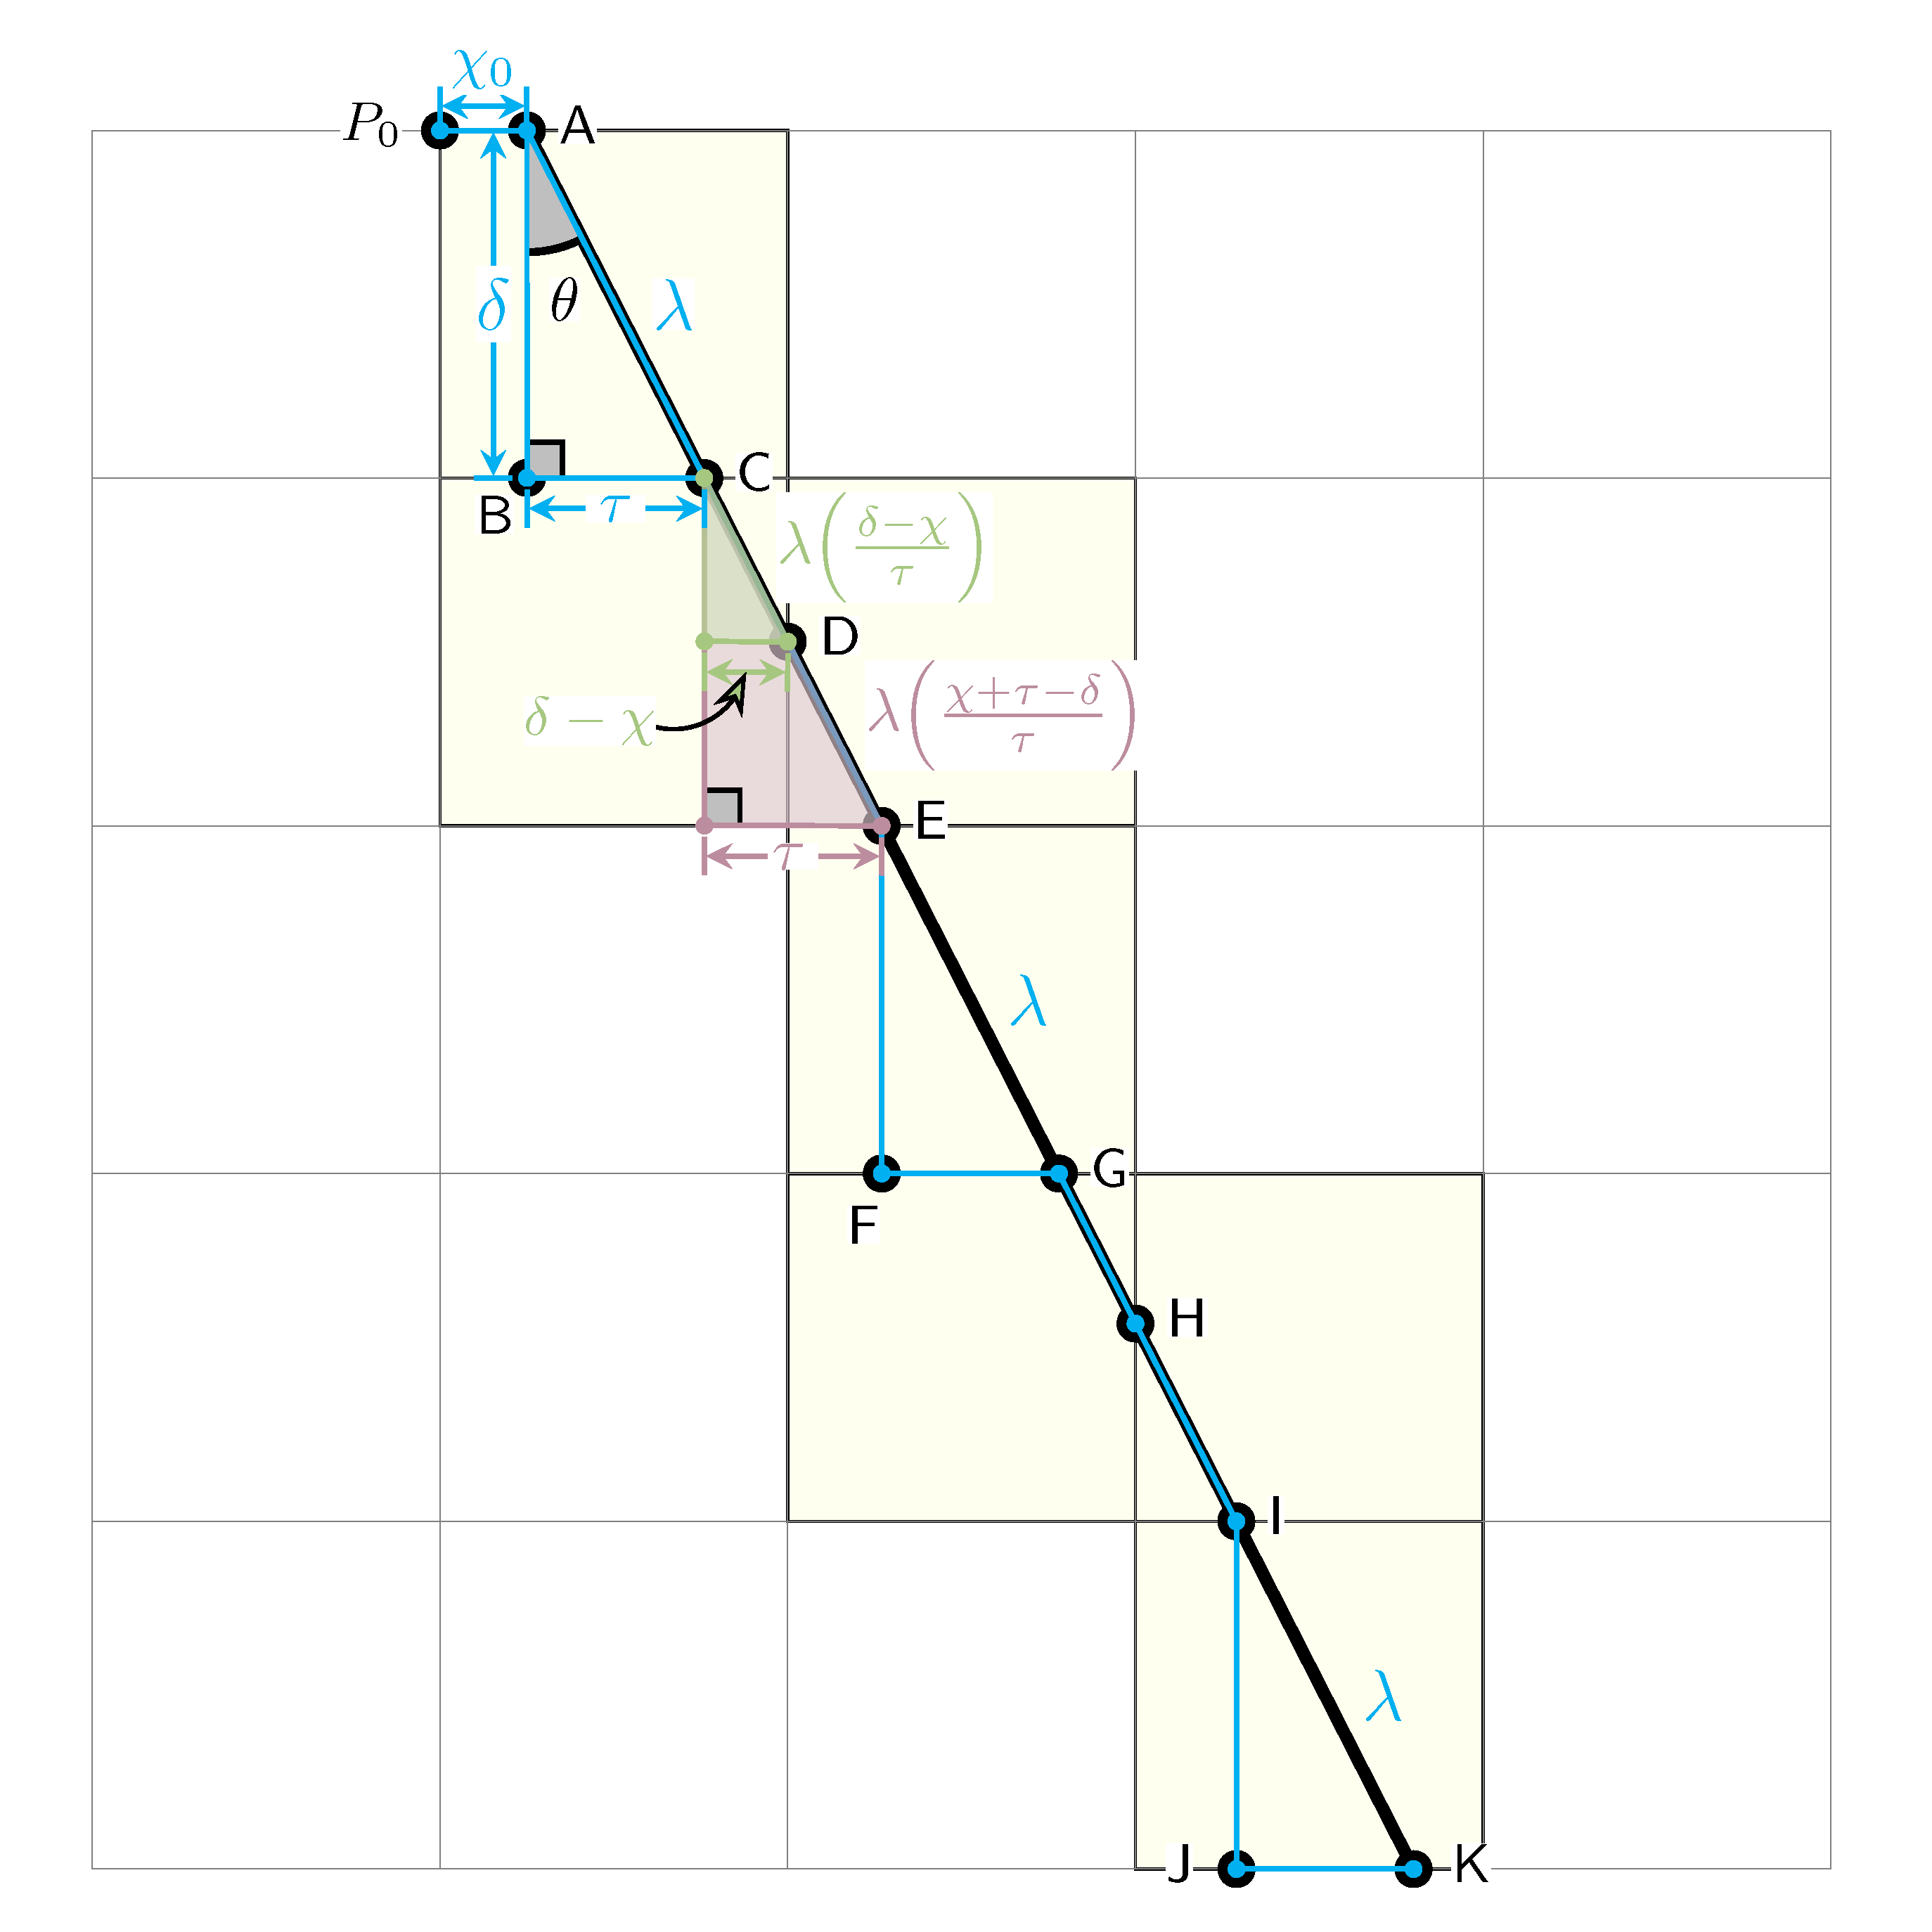
\includegraphics[width=4cm]{DDA.png}
    \caption{Hello DDA figure caption}\label{fig:DDA}
\end{figure}
%_______________________________________________________________________________________________________________________________%
%*******************************************************************************************************************************%
%===============================================================================================================================%
%------------------------------------------------ END: C2-HistoricalReview.tex -------------------------------------------------%
%===============================================================================================================================%
%*******************************************************************************************************************************%
%_______________________________________________________________________________________________________________________________%
%-------------------------------------------------------------------------------------------------------------------------------%
\endinput

	\begin{figure}
	  \centering
	  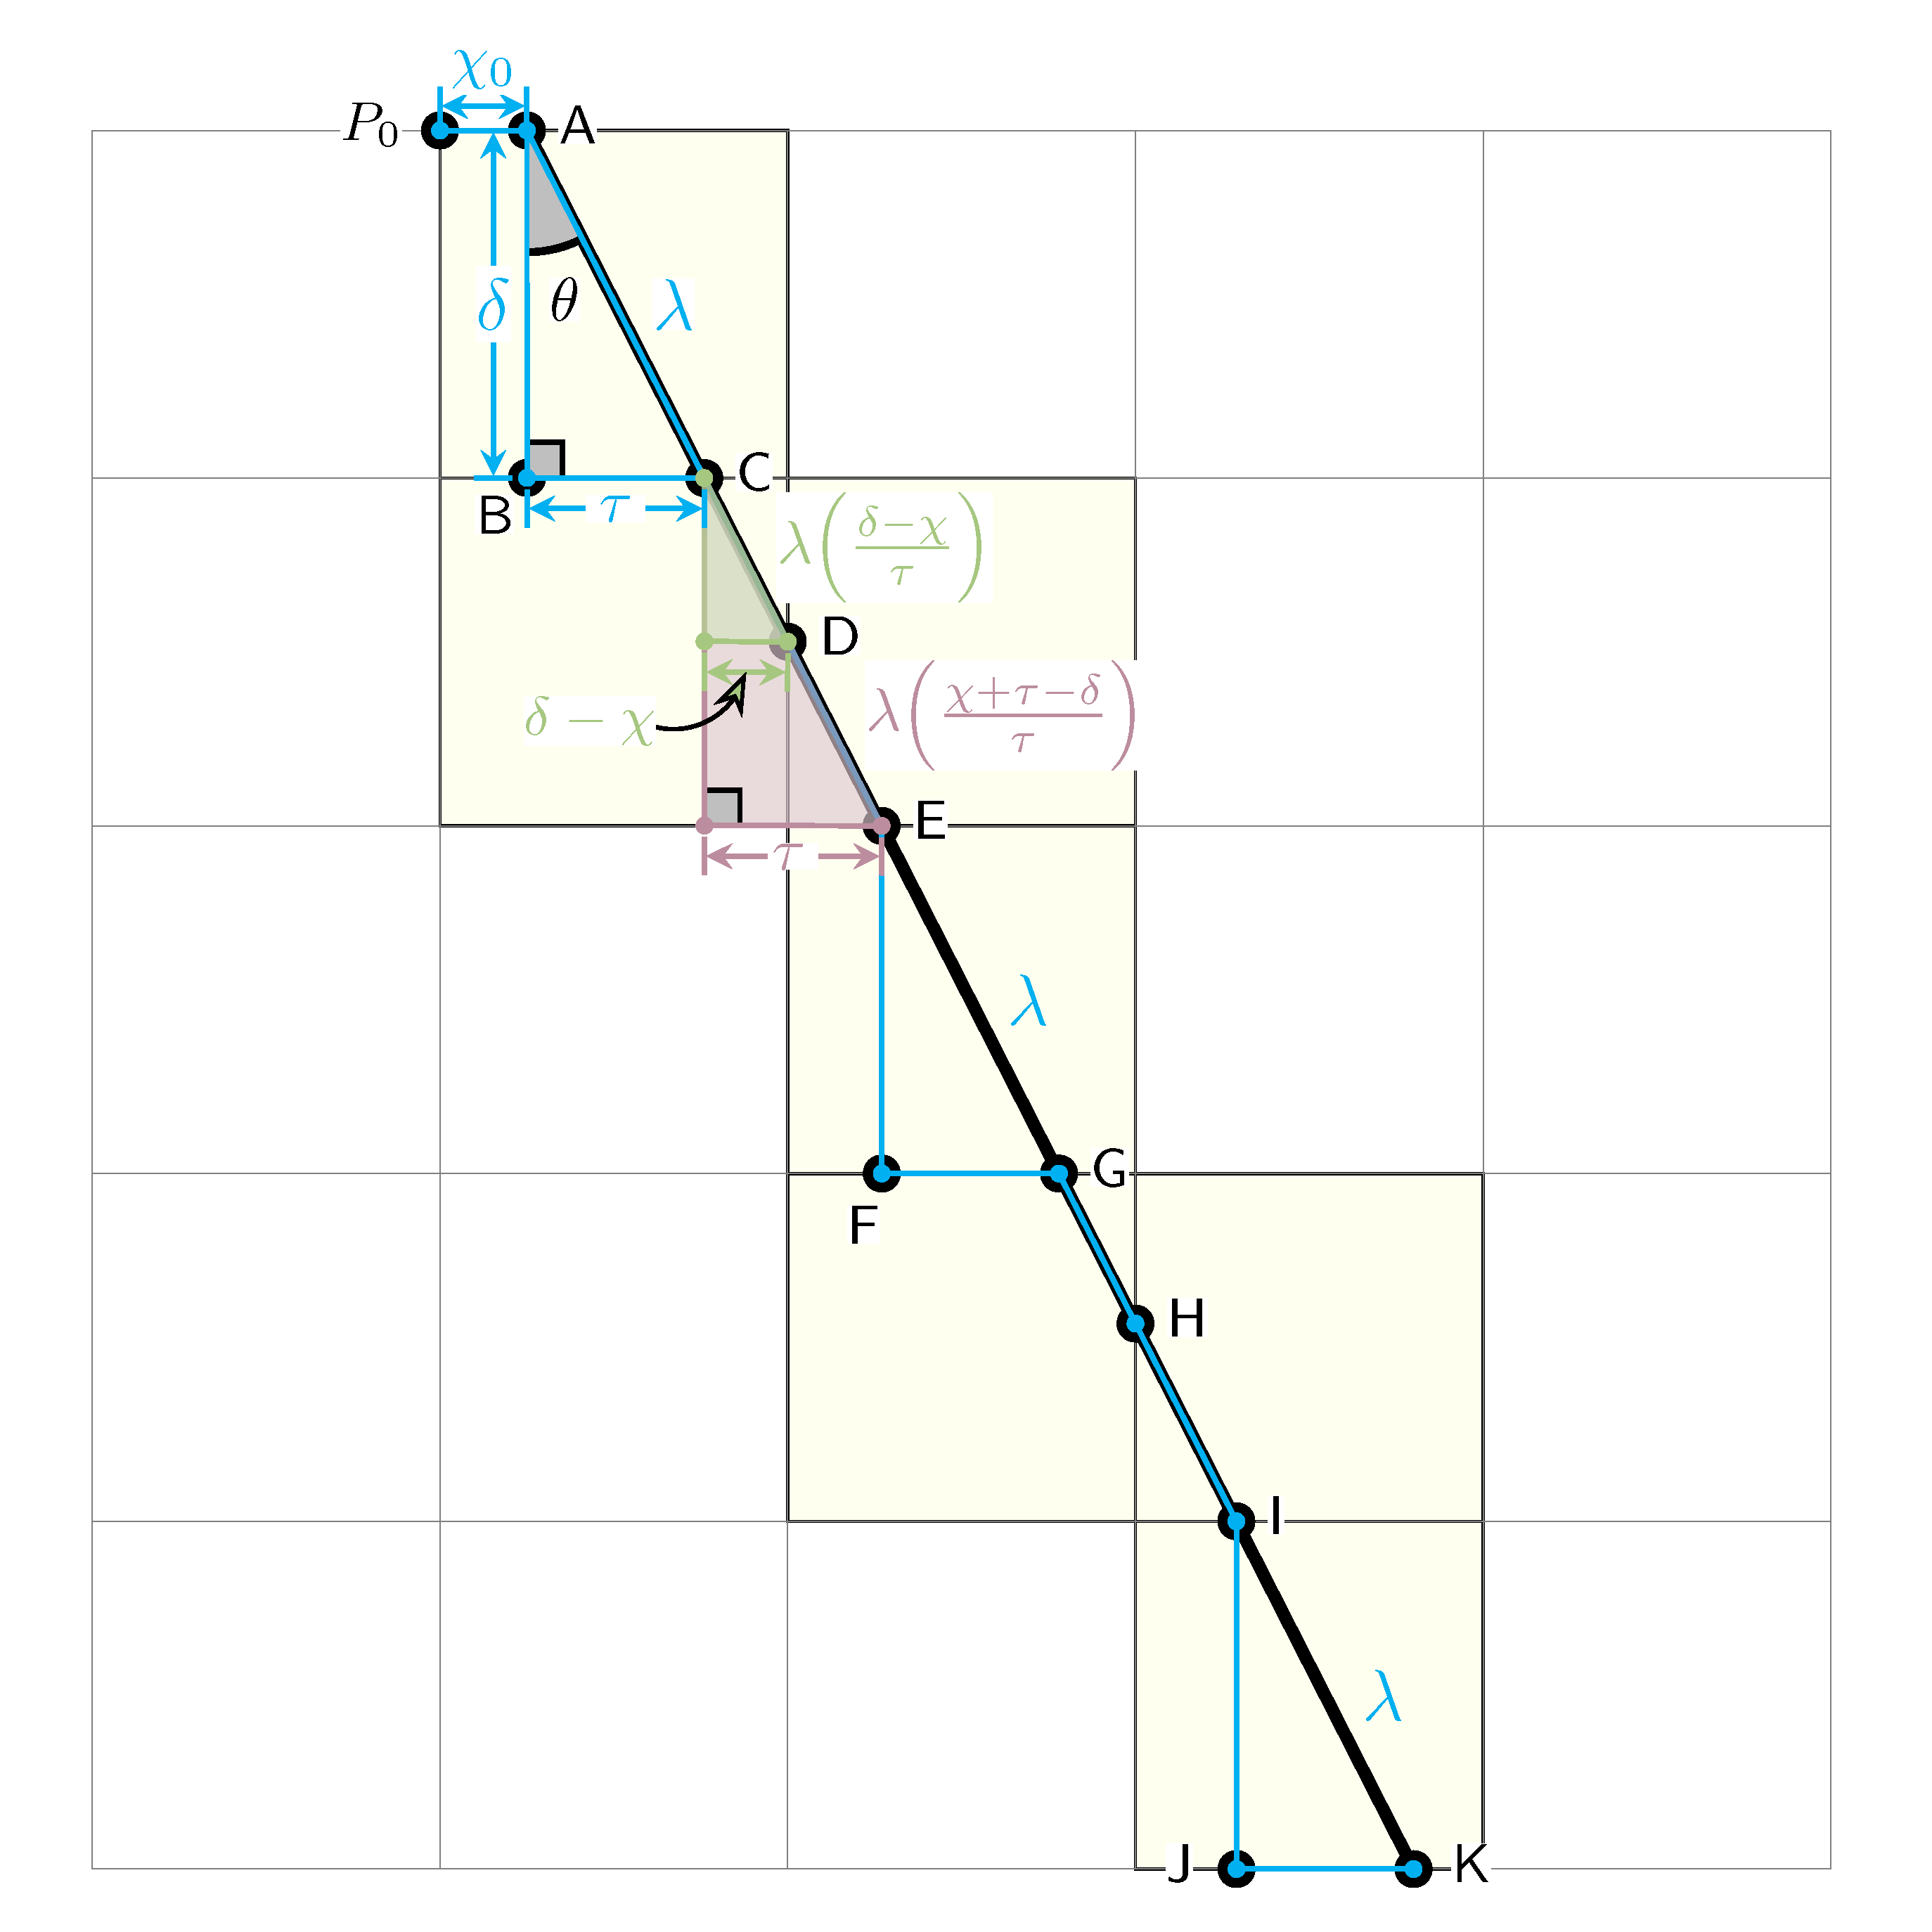
\includegraphics[width=4cm]{DDA.png}
	  \caption{Hello DDA figure caption}\label{fig:DDA}
	\end{figure}
%------------------------------------------------------------------------------------------------------------------------------%
%_______________________________________________________________________________________________________________________________%
%*******************************************************************************************************************************%
%===============================================================================================================================%
%------------------------------------------------------- C3-Methods.tex --------------------------------------------------------%
%===============================================================================================================================%
%*******************************************************************************************************************************%
%_______________________________________________________________________________________________________________________________%
%-------------------------------------------------------------------------------------------------------------------------------%
\chapter{Methods}\label{chap:methods}

Present what you did and how. May be a single Methods Chapter, or separate Methods Sections if separate topics of your dissertation are each presented as individual chapters. Alternatively, if there are methods that are relevant to all your topics, as well as methods germane to each topic individually, there might be a separate Methods Chapter here as well as Methods Sections in each topical Chapter. Cite your work where applicable~\cite{AuthorYear}.

\textbf{NOTE:} This may be broken into two chapters, e.g. '\textbf{Materials}' and '\textbf{Methods}'
%_______________________________________________________________________________________________________________________________%
%*******************************************************************************************************************************%
%===============================================================================================================================%
%----------------------------------------------------- END: C3-Methods.tex -----------------------------------------------------%
%===============================================================================================================================%
%*******************************************************************************************************************************%
%_______________________________________________________________________________________________________________________________%
%-------------------------------------------------------------------------------------------------------------------------------%
\endinput


\subappendix{explicit subappendix title (capitalized)}{%
    \label{chap3:app}
    %-------------------------------------------------------------------------------------------------------------------------------%
%~~~~~~~~~~~~~~~~~~~~~~~~~~~~~~~~~~~~~~~~~~~~~~~~~~~~~~~~~~~~~~~~~~~~~~~~~~~~~~~~~~~~~~~~~~~~~~~~~~~~~~~~~~~~~~~~~~~~~~~~~~~~~~~%
%~~~~~~~~~~~~~~~~~~~~~~~~~~~~~~~~~~~~~~~~~~~~~~~~~~~~~~~ C3-Appendix.tex ~~~~~~~~~~~~~~~~~~~~~~~~~~~~~~~~~~~~~~~~~~~~~~~~~~~~~~~%
%~~~~~~~~~~~~~~~~~~~~~~~~~~~~~~~~~~~~~~~~~~~~~~~~~~~~~~~~~~~~~~~~~~~~~~~~~~~~~~~~~~~~~~~~~~~~~~~~~~~~~~~~~~~~~~~~~~~~~~~~~~~~~~~%
%-------------------------------------------------------------------------------------------------------------------------------%

Subappendix relevant to Chapter 3 content. Material segmentation by \noexpand\section instead of by \noexpand\chapter like back matter appendices. 

The subappendices must have a level 2 title heading, which can be defined in the first parameter of the \noexpand\subappendix command (as is the case here) or defaults to ``Chapter title: Supplemental Information''if this parameter is empty. The title is automatically capitalized.
%-------------------------------------------------------------------------------------------------------------------------------%
%~~~~~~~~~~~~~~~~~~~~~~~~~~~~~~~~~~~~~~~~~~~~~~~~~~~~~~~~~~~~~~~~~~~~~~~~~~~~~~~~~~~~~~~~~~~~~~~~~~~~~~~~~~~~~~~~~~~~~~~~~~~~~~~%
%~~~~~~~~~~~~~~~~~~~~~~~~~~~~~~~~~~~~~~~~~~~~~~~~~ Appendix A-1: First Section ~~~~~~~~~~~~~~~~~~~~~~~~~~~~~~~~~~~~~~~~~~~~~~~~~%
%~~~~~~~~~~~~~~~~~~~~~~~~~~~~~~~~~~~~~~~~~~~~~~~~~~~~~~~~~~~~~~~~~~~~~~~~~~~~~~~~~~~~~~~~~~~~~~~~~~~~~~~~~~~~~~~~~~~~~~~~~~~~~~~%
%-------------------------------------------------------------------------------------------------------------------------------%
\section{First Section}\label{chap3:app:sec:one}

%-------------------------------------------------------------------------------------------------------------------------------%
%~~~~~~~~~~~~~~~~~~~~~~~~~~~~~~~~~~~~~~~~~~~~~~~~~~~~~~~~~~~~~~~~~~~~~~~~~~~~~~~~~~~~~~~~~~~~~~~~~~~~~~~~~~~~~~~~~~~~~~~~~~~~~~~%
%~~~~~~~~~~~~~~~~~~~~~~~~~~~~~~~~~~~~~~~~~~~~~~~~ Appendix A-2: Second Section ~~~~~~~~~~~~~~~~~~~~~~~~~~~~~~~~~~~~~~~~~~~~~~~~~%
%~~~~~~~~~~~~~~~~~~~~~~~~~~~~~~~~~~~~~~~~~~~~~~~~~~~~~~~~~~~~~~~~~~~~~~~~~~~~~~~~~~~~~~~~~~~~~~~~~~~~~~~~~~~~~~~~~~~~~~~~~~~~~~~%
%-------------------------------------------------------------------------------------------------------------------------------%
\section{Second Section}\label{chap3:app:sec:two}


%-------------------------------------------------------------------------------------------------------------------------------%
%*******************************************************************************************************************************%
%************************************************ END OF FILE: C3-Appendix.tex *************************************************%
%*******************************************************************************************************************************%
%-------------------------------------------------------------------------------------------------------------------------------%
\endinput

}
%------------------------------------------------------------------------------------------------------------------------------%
%_______________________________________________________________________________________________________________________________%
%*******************************************************************************************************************************%
%===============================================================================================================================%
%------------------------------------------------------- C4-Results.tex --------------------------------------------------------%
%===============================================================================================================================%
%*******************************************************************************************************************************%
%_______________________________________________________________________________________________________________________________%
%-------------------------------------------------------------------------------------------------------------------------------%
\chapter{Results}\label{chap:results}

Present the results generated using the new methods you have developed and presented here. Again, you may choose to forego a Results Chapter in favor of presenting Results Sections when individual topics of your dissertation are provided as separate chapters. In such cases, you will likely have Methods, Results and potentially Summary/Conclusion Sections in each chapter.

It is theoretically possible you may not only have Methods that are applicable to every presented (chapter) topic, but you may also have results that are applicable to every presented (chapter) topic. In that case, you could have separate Methods/Results Chapters as well as Methods/Results Sections in each Topical Chapter; the order in which the Results Chapter is included in this scenario depends on the particular scenario.

%_______________________________________________________________________________________________________________________________%
%*******************************************************************************************************************************%
%===============================================================================================================================%
%----------------------------------------------------- END: C4-Results.tex -----------------------------------------------------%
%===============================================================================================================================%
%*******************************************************************************************************************************%
%_______________________________________________________________________________________________________________________________%
%-------------------------------------------------------------------------------------------------------------------------------%
\endinput



% Empty "title" parameter -> default title inserted
\subappendix{}{%
    \label{chap4:app}
    %_______________________________________________________________________________________________________________________________%
%*******************************************************************************************************************************%
%===============================================================================================================================%
%------------------------------------------------------- C4-Appendix.tex -------------------------------------------------------%
%===============================================================================================================================%
%*******************************************************************************************************************************%
%_______________________________________________________________________________________________________________________________%
%-------------------------------------------------------------------------------------------------------------------------------%
Subappendix relevant to Chapter 4 content. In this case, the empty \noexpand\subappendix command results in the default subappendix title ``Results: Supplemental Information''.
%_______________________________________________________________________________________________________________________________%
%==============================================w================================================================================%
%------------------------------------------------- Appendix A-1: First Section -------------------------------------------------%
%===============================================================================================================================%
%_______________________________________________________________________________________________________________________________%
%-------------------------------------------------------------------------------------------------------------------------------%
\section{First Section}\label{chap4:app:sec:one}

%_______________________________________________________________________________________________________________________________%
%==============================================w================================================================================%
%------------------------------------------------ Appendix A-2: Second Section -------------------------------------------------%
%===============================================================================================================================%
%_______________________________________________________________________________________________________________________________%
%-------------------------------------------------------------------------------------------------------------------------------%
\section{Second Section}\label{chap4:app:sec:two}


%_______________________________________________________________________________________________________________________________%
%*******************************************************************************************************************************%
%===============================================================================================================================%
%---------------------------------------------------- END: C4-Appendix.tex -----------------------------------------------------%
%===============================================================================================================================%
%*******************************************************************************************************************************%
%_______________________________________________________________________________________________________________________________%
%-------------------------------------------------------------------------------------------------------------------------------%
\endinput

}
%------------------------------------------------------------------------------------------------------------------------------%
%-------------------------------------------------------------------------------------------------------------------------------%
%*******************************************************************************************************************************%
%******************************************************* C5-Summary.tex ********************************************************%
%*******************************************************************************************************************************%
%-------------------------------------------------------------------------------------------------------------------------------%
\chapter{Summary}\label{chap:summary}

Summarize and discuss results from each topic and their collective impact/importance on the field/topic. Alternatively, the summary may be combined with the conclusions to form a single Conclusion chapter.
%-------------------------------------------------------------------------------------------------------------------------------%
%*******************************************************************************************************************************%
%************************************************* END OF FILE: C5-Summary.tex *************************************************%
%*******************************************************************************************************************************%
%-------------------------------------------------------------------------------------------------------------------------------%
\endinput


%------------------------------------------------------------------------------------------------------------------------------%
%-------------------------------------------------------------------------------------------------------------------------------%
%*******************************************************************************************************************************%
%******************************************************* C5-Summary.tex ********************************************************%
%*******************************************************************************************************************************%
%-------------------------------------------------------------------------------------------------------------------------------%
\chapter{Conclusion}\label{chap:conclusion}

Provide final remarks and conclusions about the success of your work, it's contribution to the overall field/topic, and a forecast of it's importance and possible directions for future research in the particular areas presented here and/or the general field/topic. 
%-------------------------------------------------------------------------------------------------------------------------------%
%*******************************************************************************************************************************%
%************************************************* END OF FILE: C5-Summary.tex *************************************************%
%*******************************************************************************************************************************%
%-------------------------------------------------------------------------------------------------------------------------------%
\endinput


%-------------------------------------------------------------------------------------------------------------------------------%
%*******************************************************************************************************************************%
%****************************************************** BACKMATTER CONTENT *****************************************************%
%*******************************************************************************************************************************%
%-------------------------------------------------------------------------------------------------------------------------------%
%-------------------------------------------------------------------------------------------------------------------------------%
\begin{appendices}
    %\the\value{numAppendices}\\
    \chapter{Some Appendix}\label{app:a}
    Some appendix intro statement

\section[1st Appendix 1st section ToC title]{1st Appendix 1st section heading}

1st Appendix section text

\subsection[1st Appendix 1st section - 1st subsection ToC title]{1st Appendix 1st section - 1st subsection heading}

1st Appendix 1st section - 1st subsection text

\section[1st Appendix 2nd section ToC title]{1st Appendix 2nd section heading}

1st Appendix section text

\subsection[1st Appendix 2nd section - 1st subsection ToC title]{1st Appendix 2nd section - 1st subsection heading}

1st Appendix 2nd section - 1st subsection text

\endinput
    \chapter{Some Additional Appendix}\label{app:b}
    Some additional appendix intro statement

\section[2nd Appendix 1st section ToC title]{2nd Appendix 1st section heading}

1st Appendix section text

\subsection[2nd Appendix 1st section - 1st subsection ToC title]{2nd Appendix 1st section - 1st subsection heading}

1st Appendix 1st section - 1st subsection text

\section[2nd Appendix 2nd section ToC title]{2nd Appendix 2nd section heading}

2nd Appendix section text

\subsection[2nd Appendix 2nd section - 1st subsection ToC title]{2nd Appendix 2nd section - 1st subsection heading}

2nd Appendix 2nd section - 1st subsection text

\endinput
\end{appendices}
%-------------------------------------------------------------------------------------------------------------------------------%
%\bibliographystyle{chicago}                                                    % Chicago bib style
\bibliographystyle{IEEEtran}                                                    % IEEE Transactions on ... bib style
\bibliography{authors,journal-names,IEEEfull,dissertation}                      % Full IEEE/other journal names
%\bibliography{authors,journal-abrvs,IEEEabrv,pct}                              % Abbreviated IEEE/other journal names
%-------------------------------------------------------------------------------------------------------------------------------%
\end{document}
%-------------------------------------------------------------------------------------------------------------------------------%
%*******************************************************************************************************************************%
%************************************************ END: Dissertation-Schultze.tex ***********************************************%
%*******************************************************************************************************************************%
%-------------------------------------------------------------------------------------------------------------------------------%
